\documentclass[1p]{elsarticle_modified}
%\bibliographystyle{elsarticle-num}

%\usepackage[colorlinks]{hyperref}
%\usepackage{abbrmath_seonhwa} %\Abb, \Ascr, \Acal ,\Abf, \Afrak
\usepackage{amsfonts}
\usepackage{amssymb}
\usepackage{amsmath}
\usepackage{amsthm}
\usepackage{scalefnt}
\usepackage{amsbsy}
\usepackage{kotex}
\usepackage{caption}
\usepackage{subfig}
\usepackage{color}
\usepackage{graphicx}
\usepackage{xcolor} %% white, black, red, green, blue, cyan, magenta, yellow
\usepackage{float}
\usepackage{setspace}
\usepackage{hyperref}

\usepackage{tikz}
\usetikzlibrary{arrows}

\usepackage{multirow}
\usepackage{array} % fixed length table
\usepackage{hhline}

%%%%%%%%%%%%%%%%%%%%%
\makeatletter
\renewcommand*\env@matrix[1][\arraystretch]{%
	\edef\arraystretch{#1}%
	\hskip -\arraycolsep
	\let\@ifnextchar\new@ifnextchar
	\array{*\c@MaxMatrixCols c}}
\makeatother %https://tex.stackexchange.com/questions/14071/how-can-i-increase-the-line-spacing-in-a-matrix
%%%%%%%%%%%%%%%

\usepackage[normalem]{ulem}

\newcommand{\msout}[1]{\ifmmode\text{\sout{\ensuremath{#1}}}\else\sout{#1}\fi}
%SOURCE: \msout is \stkout macro in https://tex.stackexchange.com/questions/20609/strikeout-in-math-mode

\newcommand{\cancel}[1]{
	\ifmmode
	{\color{red}\msout{#1}}
	\else
	{\color{red}\sout{#1}}
	\fi
}

\newcommand{\add}[1]{
	{\color{blue}\uwave{#1}}
}

\newcommand{\replace}[2]{
	\ifmmode
	{\color{red}\msout{#1}}{\color{blue}\uwave{#2}}
	\else
	{\color{red}\sout{#1}}{\color{blue}\uwave{#2}}
	\fi
}

\newcommand{\Sol}{\mathcal{S}} %segment
\newcommand{\D}{D} %diagram
\newcommand{\A}{\mathcal{A}} %arc


%%%%%%%%%%%%%%%%%%%%%%%%%%%%%5 test

\def\sl{\operatorname{\textup{SL}}(2,\Cbb)}
\def\psl{\operatorname{\textup{PSL}}(2,\Cbb)}
\def\quan{\mkern 1mu \triangleright \mkern 1mu}

\theoremstyle{definition}
\newtheorem{thm}{Theorem}[section]
\newtheorem{prop}[thm]{Proposition}
\newtheorem{lem}[thm]{Lemma}
\newtheorem{ques}[thm]{Question}
\newtheorem{cor}[thm]{Corollary}
\newtheorem{defn}[thm]{Definition}
\newtheorem{exam}[thm]{Example}
\newtheorem{rmk}[thm]{Remark}
\newtheorem{alg}[thm]{Algorithm}

\newcommand{\I}{\sqrt{-1}}
\begin{document}

%\begin{frontmatter}
%
%\title{Boundary parabolic representations of knots up to 8 crossings}
%
%%% Group authors per affiliation:
%\author{Yunhi Cho} 
%\address{Department of Mathematics, University of Seoul, Seoul, Korea}
%\ead{yhcho@uos.ac.kr}
%
%
%\author{Seonhwa Kim} %\fnref{s_kim}}
%\address{Center for Geometry and Physics, Institute for Basic Science, Pohang, 37673, Korea}
%\ead{ryeona17@ibs.re.kr}
%
%\author{Hyuk Kim}
%\address{Department of Mathematical Sciences, Seoul National University, Seoul 08826, Korea}
%\ead{hyukkim@snu.ac.kr}
%
%\author{Seokbeom Yoon}
%\address{Department of Mathematical Sciences, Seoul National University, Seoul, 08826,  Korea}
%\ead{sbyoon15@snu.ac.kr}
%
%\begin{abstract}
%We find all boundary parabolic representation of knots up to 8 crossings.
%
%\end{abstract}
%\begin{keyword}
%    \MSC[2010] 57M25 
%\end{keyword}
%
%\end{frontmatter}

%\linenumbers
%\tableofcontents
%
\newcommand\colored[1]{\textcolor{white}{\rule[-0.35ex]{0.8em}{1.4ex}}\kern-0.8em\color{red} #1}%
%\newcommand\colored[1]{\textcolor{white}{ #1}\kern-2.17ex	\textcolor{white}{ #1}\kern-1.81ex	\textcolor{white}{ #1}\kern-2.15ex\color{red}#1	}

{\Large $\underline{12a_{0478}~(K12a_{0478})}$}

\setlength{\tabcolsep}{10pt}
\renewcommand{\arraystretch}{1.6}
\vspace{1cm}\begin{tabular}{m{100pt}>{\centering\arraybackslash}m{274pt}}
\multirow{5}{120pt}{
	\centering
	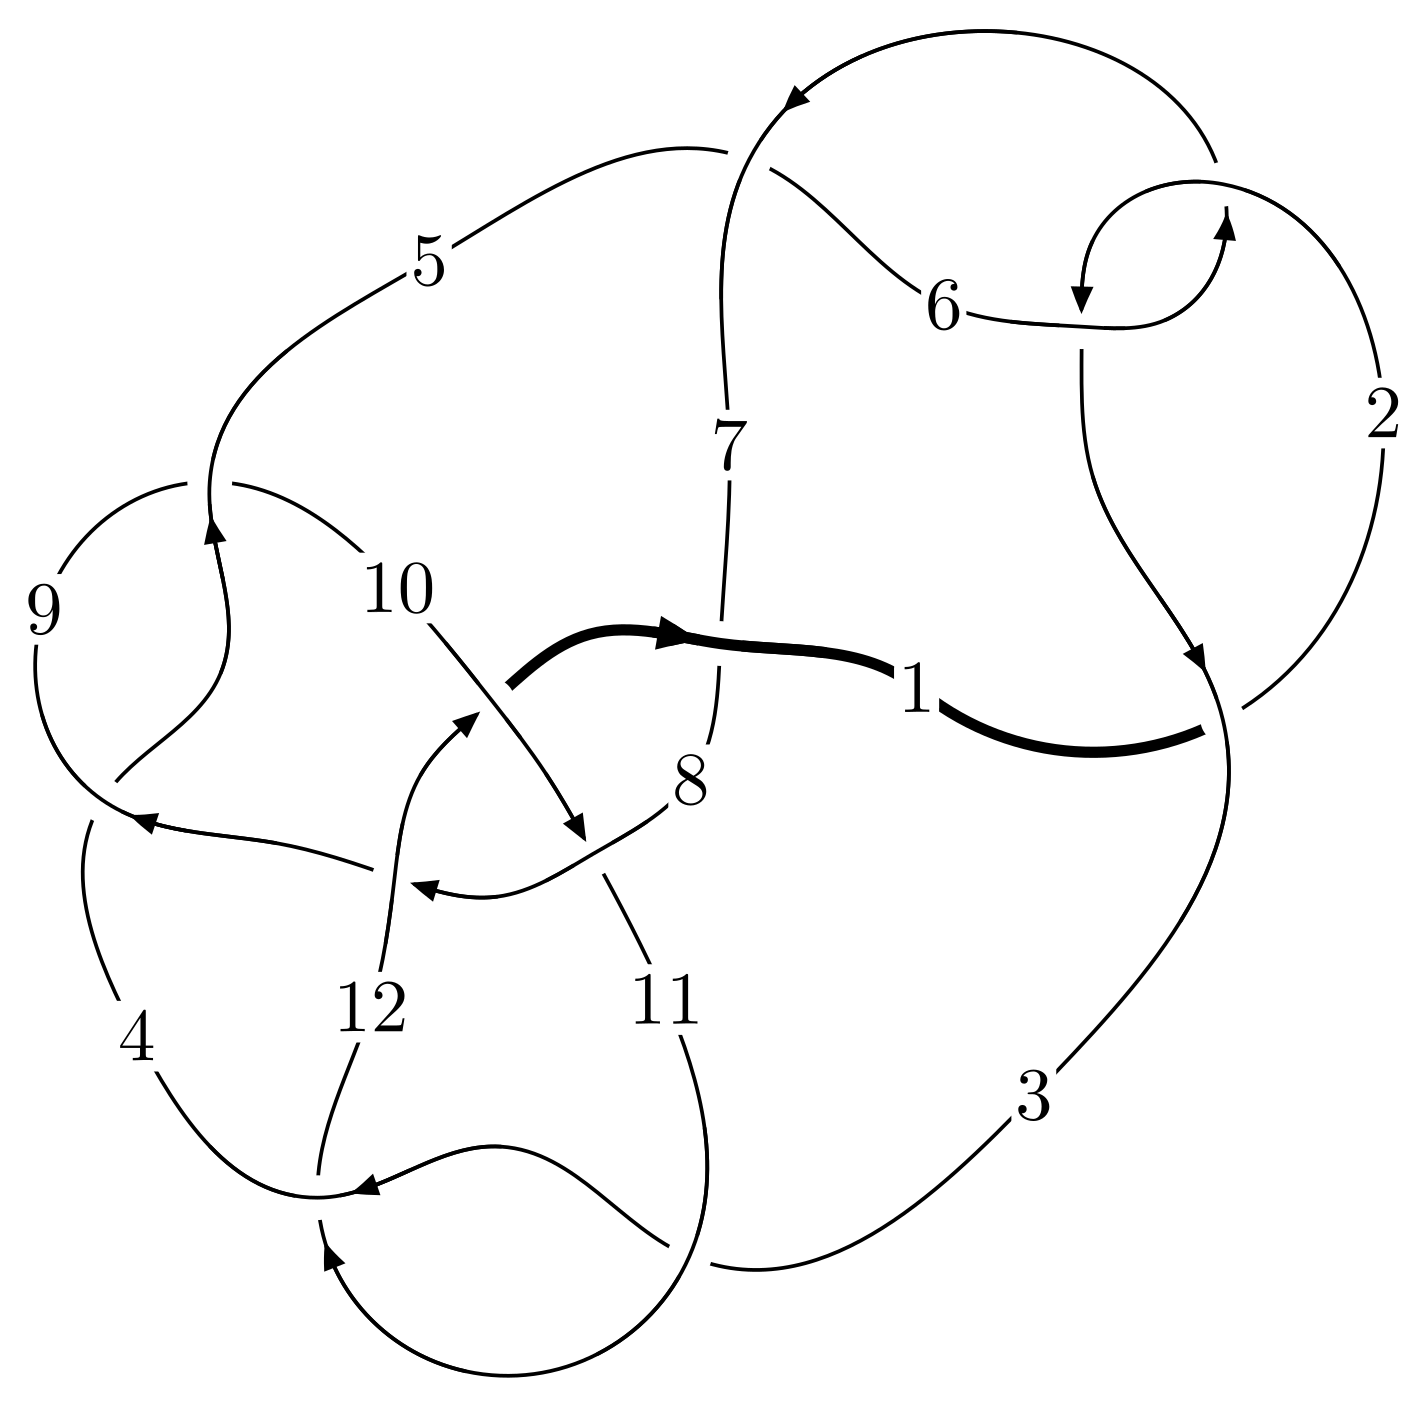
\includegraphics[width=112pt]{../../../GIT/diagram.site/Diagrams/png/1279_12a_0478.png}\\
\ \ \ A knot diagram\footnotemark}&
\allowdisplaybreaks
\textbf{Linearized knot diagam} \\
\cline{2-2}
 &
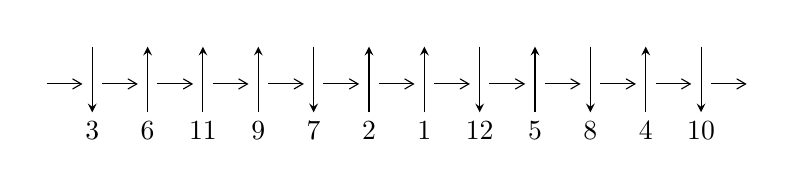
\begin{tikzpicture}[x=20pt, y=17pt]
	% nodes
	\node (C0) at (0, 0) {};
	\node (C1) at (1, 0) {};
	\node (C1U) at (1, +1) {};
	\node (C1D) at (1, -1) {3};

	\node (C2) at (2, 0) {};
	\node (C2U) at (2, +1) {};
	\node (C2D) at (2, -1) {6};

	\node (C3) at (3, 0) {};
	\node (C3U) at (3, +1) {};
	\node (C3D) at (3, -1) {11};

	\node (C4) at (4, 0) {};
	\node (C4U) at (4, +1) {};
	\node (C4D) at (4, -1) {9};

	\node (C5) at (5, 0) {};
	\node (C5U) at (5, +1) {};
	\node (C5D) at (5, -1) {7};

	\node (C6) at (6, 0) {};
	\node (C6U) at (6, +1) {};
	\node (C6D) at (6, -1) {2};

	\node (C7) at (7, 0) {};
	\node (C7U) at (7, +1) {};
	\node (C7D) at (7, -1) {1};

	\node (C8) at (8, 0) {};
	\node (C8U) at (8, +1) {};
	\node (C8D) at (8, -1) {12};

	\node (C9) at (9, 0) {};
	\node (C9U) at (9, +1) {};
	\node (C9D) at (9, -1) {5};

	\node (C10) at (10, 0) {};
	\node (C10U) at (10, +1) {};
	\node (C10D) at (10, -1) {8};

	\node (C11) at (11, 0) {};
	\node (C11U) at (11, +1) {};
	\node (C11D) at (11, -1) {4};

	\node (C12) at (12, 0) {};
	\node (C12U) at (12, +1) {};
	\node (C12D) at (12, -1) {10};
	\node (C13) at (13, 0) {};

	% arrows
	\draw[->,>={angle 60}]
	(C0) edge (C1) (C1) edge (C2) (C2) edge (C3) (C3) edge (C4) (C4) edge (C5) (C5) edge (C6) (C6) edge (C7) (C7) edge (C8) (C8) edge (C9) (C9) edge (C10) (C10) edge (C11) (C11) edge (C12) (C12) edge (C13) ;	\draw[->,>=stealth]
	(C1U) edge (C1D) (C2D) edge (C2U) (C3D) edge (C3U) (C4D) edge (C4U) (C5U) edge (C5D) (C6D) edge (C6U) (C7D) edge (C7U) (C8U) edge (C8D) (C9D) edge (C9U) (C10U) edge (C10D) (C11D) edge (C11U) (C12U) edge (C12D) ;
	\end{tikzpicture} \\
\hhline{~~} \\& 
\textbf{Solving Sequence} \\ \cline{2-2} 
 &
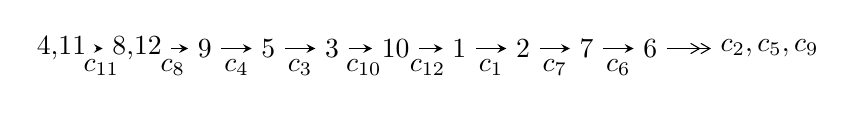
\begin{tikzpicture}[x=23pt, y=7pt]
	% node
	\node (A0) at (-1/8, 0) {4,11};
	\node (A1) at (17/16, 0) {8,12};
	\node (A2) at (17/8, 0) {9};
	\node (A3) at (25/8, 0) {5};
	\node (A4) at (33/8, 0) {3};
	\node (A5) at (41/8, 0) {10};
	\node (A6) at (49/8, 0) {1};
	\node (A7) at (57/8, 0) {2};
	\node (A8) at (65/8, 0) {7};
	\node (A9) at (73/8, 0) {6};
	\node (C1) at (1/2, -1) {$c_{11}$};
	\node (C2) at (13/8, -1) {$c_{8}$};
	\node (C3) at (21/8, -1) {$c_{4}$};
	\node (C4) at (29/8, -1) {$c_{3}$};
	\node (C5) at (37/8, -1) {$c_{10}$};
	\node (C6) at (45/8, -1) {$c_{12}$};
	\node (C7) at (53/8, -1) {$c_{1}$};
	\node (C8) at (61/8, -1) {$c_{7}$};
	\node (C9) at (69/8, -1) {$c_{6}$};
	\node (A10) at (11, 0) {$c_{2},c_{5},c_{9}$};

	% edge
	\draw[->,>=stealth]	
	(A0) edge (A1) (A1) edge (A2) (A2) edge (A3) (A3) edge (A4) (A4) edge (A5) (A5) edge (A6) (A6) edge (A7) (A7) edge (A8) (A8) edge (A9) ;
	\draw[->>,>={angle 60}]	
	(A9) edge (A10);
\end{tikzpicture} \\ 

\end{tabular} \\

\footnotetext{
The image of knot diagram is generated by the software ``\textbf{Draw programme}" developed by Andrew Bartholomew(\url{http://www.layer8.co.uk/maths/draw/index.htm\#Running-draw}), where we modified some parts for our purpose(\url{https://github.com/CATsTAILs/LinksPainter}).
}\phantom \\ \newline 
\centering \textbf{Ideals for irreducible components\footnotemark of $X_{\text{par}}$} 
 
\begin{align*}
I^u_{1}&=\langle 
5.33641\times10^{28} u^{43}-9.09644\times10^{28} u^{42}+\cdots+3.03461\times10^{30} b+1.66297\times10^{30},\\
\phantom{I^u_{1}}&\phantom{= \langle  }4.33477\times10^{29} u^{43}-4.31353\times10^{28} u^{42}+\cdots+3.03461\times10^{30} a-1.76199\times10^{30},\;u^{44}- u^{43}+\cdots+u+1\rangle \\
I^u_{2}&=\langle 
7.99621\times10^{275} u^{83}+1.94730\times10^{276} u^{82}+\cdots+8.94216\times10^{276} b-2.93848\times10^{279},\\
\phantom{I^u_{2}}&\phantom{= \langle  }-2.61794\times10^{279} u^{83}-6.34847\times10^{279} u^{82}+\cdots+2.66745\times10^{280} a+7.68018\times10^{282},\\
\phantom{I^u_{2}}&\phantom{= \langle  }u^{84}+u^{83}+\cdots+1700 u+2983\rangle \\
I^u_{3}&=\langle 
- u^2+b+1,\;u^{20}- u^{19}+\cdots+a+2,\;u^{21}- u^{20}+\cdots-3 u+1\rangle \\
\\
\end{align*}
\raggedright * 3 irreducible components of $\dim_{\mathbb{C}}=0$, with total 149 representations.\\
\footnotetext{All coefficients of polynomials are rational numbers. But the coefficients are sometimes approximated in decimal forms when there is not enough margin.}
\newpage
\renewcommand{\arraystretch}{1}
\centering \section*{I. $I^u_{1}= \langle 5.34\times10^{28} u^{43}-9.10\times10^{28} u^{42}+\cdots+3.03\times10^{30} b+1.66\times10^{30},\;4.33\times10^{29} u^{43}-4.31\times10^{28} u^{42}+\cdots+3.03\times10^{30} a-1.76\times10^{30},\;u^{44}- u^{43}+\cdots+u+1 \rangle$}
\flushleft \textbf{(i) Arc colorings}\\
\begin{tabular}{m{7pt} m{180pt} m{7pt} m{180pt} }
\flushright $a_{4}=$&$\begin{pmatrix}0\\u\end{pmatrix}$ \\
\flushright $a_{11}=$&$\begin{pmatrix}1\\0\end{pmatrix}$ \\
\flushright $a_{8}=$&$\begin{pmatrix}-0.142844 u^{43}+0.0142144 u^{42}+\cdots+1.40262 u+0.580630\\-0.0175851 u^{43}+0.0299756 u^{42}+\cdots+1.13114 u-0.548000\end{pmatrix}$ \\
\flushright $a_{12}=$&$\begin{pmatrix}1\\- u^2\end{pmatrix}$ \\
\flushright $a_{9}=$&$\begin{pmatrix}1\\-0.142844 u^{43}+0.0142144 u^{42}+\cdots+1.40262 u-0.419370\end{pmatrix}$ \\
\flushright $a_{5}=$&$\begin{pmatrix}u\\-0.128630 u^{43}+0.00337070 u^{42}+\cdots+0.723474 u+0.142844\end{pmatrix}$ \\
\flushright $a_{3}=$&$\begin{pmatrix}- u\\u\end{pmatrix}$ \\
\flushright $a_{10}=$&$\begin{pmatrix}- u^2+1\\-0.0175851 u^{43}+0.0299756 u^{42}+\cdots+1.13114 u-0.548000\end{pmatrix}$ \\
\flushright $a_{1}=$&$\begin{pmatrix}-0.000908052 u^{43}+0.108043 u^{42}+\cdots+1.12595 u+0.464391\\-0.0217088 u^{43}+0.0957979 u^{42}+\cdots-1.02492 u+0.655135\end{pmatrix}$ \\
\flushright $a_{2}=$&$\begin{pmatrix}-0.0789830 u^{43}+0.152702 u^{42}+\cdots+1.28456 u+0.645614\\0.0563662 u^{43}+0.0511385 u^{42}+\cdots-1.18352 u+0.473911\end{pmatrix}$ \\
\flushright $a_{7}=$&$\begin{pmatrix}-0.0789830 u^{43}+0.152702 u^{42}+\cdots+1.28456 u+0.645614\\-0.0516465 u^{43}-0.106716 u^{42}+\cdots+1.17971 u-0.547530\end{pmatrix}$ \\
\flushright $a_{6}=$&$\begin{pmatrix}-0.234445 u^{43}+0.296776 u^{42}+\cdots+0.343682 u+0.0836407\\0.219664 u^{43}-0.477705 u^{42}+\cdots+1.35750 u+0.331150\end{pmatrix}$\\&\end{tabular}
\flushleft \textbf{(ii) Obstruction class $= -1$}\\~\\
\flushleft \textbf{(iii) Cusp Shapes $= -0.438894 u^{43}-1.56601 u^{42}+\cdots+5.58366 u+2.74109$}\\~\\
\newpage\renewcommand{\arraystretch}{1}
\flushleft \textbf{(iv) u-Polynomials at the component}\newline \\
\begin{tabular}{m{50pt}|m{274pt}}
Crossings & \hspace{64pt}u-Polynomials at each crossing \\
\hline $$\begin{aligned}c_{1},c_{5}\end{aligned}$$&$\begin{aligned}
&u^{44}+14 u^{43}+\cdots+4 u+16
\end{aligned}$\\
\hline $$\begin{aligned}c_{2},c_{6}\end{aligned}$$&$\begin{aligned}
&u^{44}-6 u^{43}+\cdots-2 u-4
\end{aligned}$\\
\hline $$\begin{aligned}c_{3},c_{4},c_{9}\\c_{11}\end{aligned}$$&$\begin{aligned}
&u^{44}- u^{43}+\cdots+u+1
\end{aligned}$\\
\hline $$\begin{aligned}c_{7}\end{aligned}$$&$\begin{aligned}
&u^{44}+30 u^{43}+\cdots-88022 u-6988
\end{aligned}$\\
\hline $$\begin{aligned}c_{8}\end{aligned}$$&$\begin{aligned}
&u^{44}+40 u^{43}+\cdots-42991616 u-2097152
\end{aligned}$\\
\hline $$\begin{aligned}c_{10},c_{12}\end{aligned}$$&$\begin{aligned}
&u^{44}+2 u^{43}+\cdots+7 u-1
\end{aligned}$\\
\hline
\end{tabular}\\~\\
\newpage\renewcommand{\arraystretch}{1}
\flushleft \textbf{(v) Riley Polynomials at the component}\newline \\
\begin{tabular}{m{50pt}|m{274pt}}
Crossings & \hspace{64pt}Riley Polynomials at each crossing \\
\hline $$\begin{aligned}c_{1},c_{5}\end{aligned}$$&$\begin{aligned}
&y^{44}+30 y^{43}+\cdots+9744 y+256
\end{aligned}$\\
\hline $$\begin{aligned}c_{2},c_{6}\end{aligned}$$&$\begin{aligned}
&y^{44}+14 y^{43}+\cdots+4 y+16
\end{aligned}$\\
\hline $$\begin{aligned}c_{3},c_{4},c_{9}\\c_{11}\end{aligned}$$&$\begin{aligned}
&y^{44}-31 y^{43}+\cdots+y+1
\end{aligned}$\\
\hline $$\begin{aligned}c_{7}\end{aligned}$$&$\begin{aligned}
&y^{44}+6 y^{43}+\cdots+106960964 y+48832144
\end{aligned}$\\
\hline $$\begin{aligned}c_{8}\end{aligned}$$&$\begin{aligned}
&y^{44}-2 y^{43}+\cdots-7696581394432 y+4398046511104
\end{aligned}$\\
\hline $$\begin{aligned}c_{10},c_{12}\end{aligned}$$&$\begin{aligned}
&y^{44}-10 y^{43}+\cdots-37 y+1
\end{aligned}$\\
\hline
\end{tabular}\\~\\
\newpage\flushleft \textbf{(vi) Complex Volumes and Cusp Shapes}
$$\begin{array}{c|c|c}  
\text{Solutions to }I^u_{1}& \I (\text{vol} + \sqrt{-1}CS) & \text{Cusp shape}\\
 \hline 
\begin{aligned}
u &= \phantom{-}0.963533 + 0.350253 I \\
a &= \phantom{-}0.86851 + 1.90330 I \\
b &= \phantom{-}0.453390 - 0.216435 I\end{aligned}
 & \phantom{-}3.18342 + 3.22741 I & \phantom{-}0.25538 - 6.57497 I \\ \hline\begin{aligned}
u &= \phantom{-}0.963533 - 0.350253 I \\
a &= \phantom{-}0.86851 - 1.90330 I \\
b &= \phantom{-}0.453390 + 0.216435 I\end{aligned}
 & \phantom{-}3.18342 - 3.22741 I & \phantom{-}0.25538 + 6.57497 I \\ \hline\begin{aligned}
u &= -1.022440 + 0.093582 I \\
a &= -0.935498 + 0.358789 I \\
b &= -1.034400 - 0.192161 I\end{aligned}
 & -1.47417 - 3.43532 I & \phantom{-}0.66881 + 5.03721 I \\ \hline\begin{aligned}
u &= -1.022440 - 0.093582 I \\
a &= -0.935498 - 0.358789 I \\
b &= -1.034400 + 0.192161 I\end{aligned}
 & -1.47417 + 3.43532 I & \phantom{-}0.66881 - 5.03721 I \\ \hline\begin{aligned}
u &= \phantom{-}1.05616\phantom{ +0.000000I} \\
a &= -1.31524\phantom{ +0.000000I} \\
b &= -0.848120\phantom{ +0.000000I}\end{aligned}
 & \phantom{-}2.23451\phantom{ +0.000000I} & \phantom{-}3.56780\phantom{ +0.000000I} \\ \hline\begin{aligned}
u &= -0.980841 + 0.478403 I \\
a &= \phantom{-}0.65210 - 1.59072 I \\
b &= \phantom{-}0.666848 + 0.187542 I\end{aligned}
 & \phantom{-}1.53255 - 8.57516 I & \phantom{-}0.51722 + 9.73471 I \\ \hline\begin{aligned}
u &= -0.980841 - 0.478403 I \\
a &= \phantom{-}0.65210 + 1.59072 I \\
b &= \phantom{-}0.666848 - 0.187542 I\end{aligned}
 & \phantom{-}1.53255 + 8.57516 I & \phantom{-}0.51722 - 9.73471 I \\ \hline\begin{aligned}
u &= \phantom{-}1.139270 + 0.093898 I \\
a &= -1.058050 - 0.808186 I \\
b &= -0.866999 + 0.460040 I\end{aligned}
 & \phantom{-}6.02381 + 3.30020 I & \phantom{-}7.56096 - 4.45656 I \\ \hline\begin{aligned}
u &= \phantom{-}1.139270 - 0.093898 I \\
a &= -1.058050 + 0.808186 I \\
b &= -0.866999 - 0.460040 I\end{aligned}
 & \phantom{-}6.02381 - 3.30020 I & \phantom{-}7.56096 + 4.45656 I \\ \hline\begin{aligned}
u &= -1.143130 + 0.125355 I \\
a &= -0.938693 + 0.792091 I \\
b &= -0.953820 - 0.499545 I\end{aligned}
 & \phantom{-}4.99041 - 9.37474 I & \phantom{-}6.29693 + 8.40216 I\\
 \hline 
 \end{array}$$\newpage$$\begin{array}{c|c|c}  
\text{Solutions to }I^u_{1}& \I (\text{vol} + \sqrt{-1}CS) & \text{Cusp shape}\\
 \hline 
\begin{aligned}
u &= -1.143130 - 0.125355 I \\
a &= -0.938693 - 0.792091 I \\
b &= -0.953820 + 0.499545 I\end{aligned}
 & \phantom{-}4.99041 + 9.37474 I & \phantom{-}6.29693 - 8.40216 I \\ \hline\begin{aligned}
u &= \phantom{-}0.217696 + 0.819184 I \\
a &= \phantom{-}0.152694 - 0.527270 I \\
b &= -0.940135 - 0.910573 I\end{aligned}
 & -0.52383 - 7.78712 I & \phantom{-}0.00351 + 6.35147 I \\ \hline\begin{aligned}
u &= \phantom{-}0.217696 - 0.819184 I \\
a &= \phantom{-}0.152694 + 0.527270 I \\
b &= -0.940135 + 0.910573 I\end{aligned}
 & -0.52383 + 7.78712 I & \phantom{-}0.00351 - 6.35147 I \\ \hline\begin{aligned}
u &= -0.688920 + 0.451970 I \\
a &= \phantom{-}1.02687 - 1.08790 I \\
b &= \phantom{-}0.426757 - 0.154326 I\end{aligned}
 & -2.73346 - 2.08740 I & -3.07292 + 2.85449 I \\ \hline\begin{aligned}
u &= -0.688920 - 0.451970 I \\
a &= \phantom{-}1.02687 + 1.08790 I \\
b &= \phantom{-}0.426757 + 0.154326 I\end{aligned}
 & -2.73346 + 2.08740 I & -3.07292 - 2.85449 I \\ \hline\begin{aligned}
u &= -0.176839 + 0.789101 I \\
a &= \phantom{-}0.180681 + 0.508444 I \\
b &= -0.854363 + 0.859568 I\end{aligned}
 & \phantom{-}0.40669 + 2.26076 I & \phantom{-}1.58718 - 1.55987 I \\ \hline\begin{aligned}
u &= -0.176839 - 0.789101 I \\
a &= \phantom{-}0.180681 - 0.508444 I \\
b &= -0.854363 - 0.859568 I\end{aligned}
 & \phantom{-}0.40669 - 2.26076 I & \phantom{-}1.58718 + 1.55987 I \\ \hline\begin{aligned}
u &= \phantom{-}0.308970 + 0.711810 I \\
a &= \phantom{-}0.086084 - 0.461553 I \\
b &= -1.081530 - 0.689213 I\end{aligned}
 & -5.25526 - 2.25847 I & -6.26530 + 1.17443 I \\ \hline\begin{aligned}
u &= \phantom{-}0.308970 - 0.711810 I \\
a &= \phantom{-}0.086084 + 0.461553 I \\
b &= -1.081530 + 0.689213 I\end{aligned}
 & -5.25526 + 2.25847 I & -6.26530 - 1.17443 I \\ \hline\begin{aligned}
u &= -0.364868 + 0.635114 I \\
a &= \phantom{-}0.660022 - 0.672984 I \\
b &= \phantom{-}0.150292 - 0.548954 I\end{aligned}
 & \phantom{-}0.83408 + 3.47441 I & \phantom{-}2.06056 - 1.25791 I\\
 \hline 
 \end{array}$$\newpage$$\begin{array}{c|c|c}  
\text{Solutions to }I^u_{1}& \I (\text{vol} + \sqrt{-1}CS) & \text{Cusp shape}\\
 \hline 
\begin{aligned}
u &= -0.364868 - 0.635114 I \\
a &= \phantom{-}0.660022 + 0.672984 I \\
b &= \phantom{-}0.150292 + 0.548954 I\end{aligned}
 & \phantom{-}0.83408 - 3.47441 I & \phantom{-}2.06056 + 1.25791 I \\ \hline\begin{aligned}
u &= \phantom{-}0.457923 + 0.566781 I \\
a &= -0.044360 - 0.398417 I \\
b &= -1.256120 - 0.419833 I\end{aligned}
 & -2.07652 + 3.22600 I & -0.64383 - 7.61023 I \\ \hline\begin{aligned}
u &= \phantom{-}0.457923 - 0.566781 I \\
a &= -0.044360 + 0.398417 I \\
b &= -1.256120 + 0.419833 I\end{aligned}
 & -2.07652 - 3.22600 I & -0.64383 + 7.61023 I \\ \hline\begin{aligned}
u &= \phantom{-}0.236575 + 0.631412 I \\
a &= \phantom{-}0.581720 + 0.550322 I \\
b &= -0.054507 + 0.565134 I\end{aligned}
 & \phantom{-}1.51179 + 1.75801 I & \phantom{-}3.42715 - 4.74250 I \\ \hline\begin{aligned}
u &= \phantom{-}0.236575 - 0.631412 I \\
a &= \phantom{-}0.581720 - 0.550322 I \\
b &= -0.054507 - 0.565134 I\end{aligned}
 & \phantom{-}1.51179 - 1.75801 I & \phantom{-}3.42715 + 4.74250 I \\ \hline\begin{aligned}
u &= \phantom{-}0.645516\phantom{ +0.000000I} \\
a &= \phantom{-}2.06097\phantom{ +0.000000I} \\
b &= \phantom{-}0.202182\phantom{ +0.000000I}\end{aligned}
 & \phantom{-}1.23926\phantom{ +0.000000I} & \phantom{-}13.0470\phantom{ +0.000000I} \\ \hline\begin{aligned}
u &= \phantom{-}1.348290 + 0.336035 I \\
a &= -0.06962 + 1.61677 I \\
b &= \phantom{-}0.514106 - 1.076690 I\end{aligned}
 & \phantom{-}11.66130 + 2.70389 I & \phantom{-0.000000 } 0 \\ \hline\begin{aligned}
u &= \phantom{-}1.348290 - 0.336035 I \\
a &= -0.06962 - 1.61677 I \\
b &= \phantom{-}0.514106 + 1.076690 I\end{aligned}
 & \phantom{-}11.66130 - 2.70389 I & \phantom{-0.000000 } 0 \\ \hline\begin{aligned}
u &= -0.461955 + 0.387848 I \\
a &= -0.104836 + 0.279406 I \\
b &= -1.198360 + 0.224243 I\end{aligned}
 & -1.42861 + 1.53127 I & \phantom{-}2.46911 + 4.30137 I \\ \hline\begin{aligned}
u &= -0.461955 - 0.387848 I \\
a &= -0.104836 - 0.279406 I \\
b &= -1.198360 - 0.224243 I\end{aligned}
 & -1.42861 - 1.53127 I & \phantom{-}2.46911 - 4.30137 I\\
 \hline 
 \end{array}$$\newpage$$\begin{array}{c|c|c}  
\text{Solutions to }I^u_{1}& \I (\text{vol} + \sqrt{-1}CS) & \text{Cusp shape}\\
 \hline 
\begin{aligned}
u &= \phantom{-}1.31771 + 0.52143 I \\
a &= \phantom{-}0.13723 + 1.49979 I \\
b &= \phantom{-}0.997246 - 0.885207 I\end{aligned}
 & \phantom{-}3.63174 + 5.85824 I & \phantom{-0.000000 } 0 \\ \hline\begin{aligned}
u &= \phantom{-}1.31771 - 0.52143 I \\
a &= \phantom{-}0.13723 - 1.49979 I \\
b &= \phantom{-}0.997246 + 0.885207 I\end{aligned}
 & \phantom{-}3.63174 - 5.85824 I & \phantom{-0.000000 } 0 \\ \hline\begin{aligned}
u &= -1.37313 + 0.36438 I \\
a &= -0.04599 - 1.56888 I \\
b &= \phantom{-}0.604568 + 1.134910 I\end{aligned}
 & \phantom{-}11.8635 - 8.8046 I & \phantom{-0.000000 } 0 \\ \hline\begin{aligned}
u &= -1.37313 - 0.36438 I \\
a &= -0.04599 + 1.56888 I \\
b &= \phantom{-}0.604568 - 1.134910 I\end{aligned}
 & \phantom{-}11.8635 + 8.8046 I & \phantom{-0.000000 } 0 \\ \hline\begin{aligned}
u &= -0.153275 + 0.539163 I \\
a &= \phantom{-}0.183448 + 0.292807 I \\
b &= -0.815929 + 0.401366 I\end{aligned}
 & -1.39440 + 1.01413 I & -2.43614 - 1.49783 I \\ \hline\begin{aligned}
u &= -0.153275 - 0.539163 I \\
a &= \phantom{-}0.183448 - 0.292807 I \\
b &= -0.815929 - 0.401366 I\end{aligned}
 & -1.39440 - 1.01413 I & -2.43614 + 1.49783 I \\ \hline\begin{aligned}
u &= -1.38286 + 0.50685 I \\
a &= \phantom{-}0.07770 - 1.47027 I \\
b &= \phantom{-}1.01010 + 1.07254 I\end{aligned}
 & \phantom{-}6.12470 - 9.94560 I & \phantom{-0.000000 } 0 \\ \hline\begin{aligned}
u &= -1.38286 - 0.50685 I \\
a &= \phantom{-}0.07770 + 1.47027 I \\
b &= \phantom{-}1.01010 - 1.07254 I\end{aligned}
 & \phantom{-}6.12470 + 9.94560 I & \phantom{-0.000000 } 0 \\ \hline\begin{aligned}
u &= \phantom{-}1.40141 + 0.56071 I \\
a &= \phantom{-}0.09688 + 1.42482 I \\
b &= \phantom{-}1.17626 - 1.07775 I\end{aligned}
 & \phantom{-}1.86199 + 12.59430 I & \phantom{-0.000000 } 0 \\ \hline\begin{aligned}
u &= \phantom{-}1.40141 - 0.56071 I \\
a &= \phantom{-}0.09688 - 1.42482 I \\
b &= \phantom{-}1.17626 + 1.07775 I\end{aligned}
 & \phantom{-}1.86199 - 12.59430 I & \phantom{-0.000000 } 0\\
 \hline 
 \end{array}$$\newpage$$\begin{array}{c|c|c}  
\text{Solutions to }I^u_{1}& \I (\text{vol} + \sqrt{-1}CS) & \text{Cusp shape}\\
 \hline 
\begin{aligned}
u &= -1.45240 + 0.53962 I \\
a &= \phantom{-}0.057156 - 1.409450 I \\
b &= \phantom{-}1.16253 + 1.24292 I\end{aligned}
 & \phantom{-}8.6839 - 12.8336 I & \phantom{-0.000000 } 0 \\ \hline\begin{aligned}
u &= -1.45240 - 0.53962 I \\
a &= \phantom{-}0.057156 + 1.409450 I \\
b &= \phantom{-}1.16253 - 1.24292 I\end{aligned}
 & \phantom{-}8.6839 + 12.8336 I & \phantom{-0.000000 } 0 \\ \hline\begin{aligned}
u &= \phantom{-}1.45843 + 0.55635 I \\
a &= \phantom{-}0.063082 + 1.397950 I \\
b &= \phantom{-}1.21703 - 1.24520 I\end{aligned}
 & \phantom{-}7.5897 + 18.7123 I & \phantom{-0.000000 } 0 \\ \hline\begin{aligned}
u &= \phantom{-}1.45843 - 0.55635 I \\
a &= \phantom{-}0.063082 - 1.397950 I \\
b &= \phantom{-}1.21703 + 1.24520 I\end{aligned}
 & \phantom{-}7.5897 - 18.7123 I & \phantom{-0.000000 } 0\\
 \hline 
 \end{array}$$\newpage\newpage\renewcommand{\arraystretch}{1}
\centering \section*{II. $I^u_{2}= \langle 8.00\times10^{275} u^{83}+1.95\times10^{276} u^{82}+\cdots+8.94\times10^{276} b-2.94\times10^{279},\;-2.62\times10^{279} u^{83}-6.35\times10^{279} u^{82}+\cdots+2.67\times10^{280} a+7.68\times10^{282},\;u^{84}+u^{83}+\cdots+1700 u+2983 \rangle$}
\flushleft \textbf{(i) Arc colorings}\\
\begin{tabular}{m{7pt} m{180pt} m{7pt} m{180pt} }
\flushright $a_{4}=$&$\begin{pmatrix}0\\u\end{pmatrix}$ \\
\flushright $a_{11}=$&$\begin{pmatrix}1\\0\end{pmatrix}$ \\
\flushright $a_{8}=$&$\begin{pmatrix}0.0981441 u^{83}+0.237998 u^{82}+\cdots-461.448 u-287.922\\-0.0894214 u^{83}-0.217766 u^{82}+\cdots+415.217 u+328.609\end{pmatrix}$ \\
\flushright $a_{12}=$&$\begin{pmatrix}1\\- u^2\end{pmatrix}$ \\
\flushright $a_{9}=$&$\begin{pmatrix}0.0717702 u^{83}+0.154245 u^{82}+\cdots-346.149 u-199.348\\-0.0466237 u^{83}-0.0835566 u^{82}+\cdots+238.998 u+157.447\end{pmatrix}$ \\
\flushright $a_{5}=$&$\begin{pmatrix}-0.180265 u^{83}-0.321728 u^{82}+\cdots+766.751 u+328.107\\0.174737 u^{83}+0.332085 u^{82}+\cdots-717.974 u-456.666\end{pmatrix}$ \\
\flushright $a_{3}=$&$\begin{pmatrix}- u\\u\end{pmatrix}$ \\
\flushright $a_{10}=$&$\begin{pmatrix}-0.180348 u^{83}-0.497384 u^{82}+\cdots+739.524 u+644.660\\0.251112 u^{83}+0.641466 u^{82}+\cdots-1096.60 u-894.041\end{pmatrix}$ \\
\flushright $a_{1}=$&$\begin{pmatrix}0.170906 u^{83}+0.314317 u^{82}+\cdots-852.555 u-530.571\\-0.0636915 u^{83}-0.0558300 u^{82}+\cdots+362.180 u+134.499\end{pmatrix}$ \\
\flushright $a_{2}=$&$\begin{pmatrix}0.0385080 u^{83}-0.00797016 u^{82}+\cdots-275.571 u-79.3238\\0.0687064 u^{83}+0.266457 u^{82}+\cdots-214.804 u-316.748\end{pmatrix}$ \\
\flushright $a_{7}=$&$\begin{pmatrix}-0.0970944 u^{83}-0.280754 u^{82}+\cdots+381.748 u+372.199\\0.285872 u^{83}+0.718243 u^{82}+\cdots-1158.87 u-926.093\end{pmatrix}$ \\
\flushright $a_{6}=$&$\begin{pmatrix}0.504901 u^{83}+0.999388 u^{82}+\cdots-1864.77 u-1209.57\\-0.399278 u^{83}-0.751070 u^{82}+\cdots+1389.21 u+833.181\end{pmatrix}$\\&\end{tabular}
\flushleft \textbf{(ii) Obstruction class $= -1$}\\~\\
\flushleft \textbf{(iii) Cusp Shapes $= -0.529975 u^{83}-1.07671 u^{82}+\cdots+1915.72 u+1175.59$}\\~\\
\newpage\renewcommand{\arraystretch}{1}
\flushleft \textbf{(iv) u-Polynomials at the component}\newline \\
\begin{tabular}{m{50pt}|m{274pt}}
Crossings & \hspace{64pt}u-Polynomials at each crossing \\
\hline $$\begin{aligned}c_{1},c_{5}\end{aligned}$$&$\begin{aligned}
&(u^{21}+7 u^{20}+\cdots+3 u-1)^{4}
\end{aligned}$\\
\hline $$\begin{aligned}c_{2},c_{6}\end{aligned}$$&$\begin{aligned}
&(u^{21}+u^{20}+\cdots+u+1)^{4}
\end{aligned}$\\
\hline $$\begin{aligned}c_{3},c_{4},c_{9}\\c_{11}\end{aligned}$$&$\begin{aligned}
&u^{84}+u^{83}+\cdots+1700 u+2983
\end{aligned}$\\
\hline $$\begin{aligned}c_{7}\end{aligned}$$&$\begin{aligned}
&(u^{21}-5 u^{20}+\cdots-11 u+3)^{4}
\end{aligned}$\\
\hline $$\begin{aligned}c_{8}\end{aligned}$$&$\begin{aligned}
&(u^2- u+1)^{42}
\end{aligned}$\\
\hline $$\begin{aligned}c_{10},c_{12}\end{aligned}$$&$\begin{aligned}
&u^{84}-23 u^{83}+\cdots-646 u+37
\end{aligned}$\\
\hline
\end{tabular}\\~\\
\newpage\renewcommand{\arraystretch}{1}
\flushleft \textbf{(v) Riley Polynomials at the component}\newline \\
\begin{tabular}{m{50pt}|m{274pt}}
Crossings & \hspace{64pt}Riley Polynomials at each crossing \\
\hline $$\begin{aligned}c_{1},c_{5}\end{aligned}$$&$\begin{aligned}
&(y^{21}+15 y^{20}+\cdots+27 y-1)^{4}
\end{aligned}$\\
\hline $$\begin{aligned}c_{2},c_{6}\end{aligned}$$&$\begin{aligned}
&(y^{21}+7 y^{20}+\cdots+3 y-1)^{4}
\end{aligned}$\\
\hline $$\begin{aligned}c_{3},c_{4},c_{9}\\c_{11}\end{aligned}$$&$\begin{aligned}
&y^{84}-69 y^{83}+\cdots-605825892 y+8898289
\end{aligned}$\\
\hline $$\begin{aligned}c_{7}\end{aligned}$$&$\begin{aligned}
&(y^{21}+3 y^{20}+\cdots-41 y-9)^{4}
\end{aligned}$\\
\hline $$\begin{aligned}c_{8}\end{aligned}$$&$\begin{aligned}
&(y^2+y+1)^{42}
\end{aligned}$\\
\hline $$\begin{aligned}c_{10},c_{12}\end{aligned}$$&$\begin{aligned}
&y^{84}+19 y^{83}+\cdots+39856 y+1369
\end{aligned}$\\
\hline
\end{tabular}\\~\\
\newpage\flushleft \textbf{(vi) Complex Volumes and Cusp Shapes}
$$\begin{array}{c|c|c}  
\text{Solutions to }I^u_{2}& \I (\text{vol} + \sqrt{-1}CS) & \text{Cusp shape}\\
 \hline 
\begin{aligned}
u &= \phantom{-}0.601980 + 0.847982 I \\
a &= -0.395112 + 0.064605 I \\
b &= \phantom{-}0.425024 - 0.439597 I\end{aligned}
 & \phantom{-}6.30468 + 4.71576 I & \phantom{-0.000000 } 0 \\ \hline\begin{aligned}
u &= \phantom{-}0.601980 - 0.847982 I \\
a &= -0.395112 - 0.064605 I \\
b &= \phantom{-}0.425024 + 0.439597 I\end{aligned}
 & \phantom{-}6.30468 - 4.71576 I & \phantom{-0.000000 } 0 \\ \hline\begin{aligned}
u &= -0.768780 + 0.567617 I \\
a &= \phantom{-}0.943793 - 0.486452 I \\
b &= \phantom{-}0.670826 + 0.088440 I\end{aligned}
 & -2.65275 - 2.26732 I & \phantom{-0.000000 } 0 \\ \hline\begin{aligned}
u &= -0.768780 - 0.567617 I \\
a &= \phantom{-}0.943793 + 0.486452 I \\
b &= \phantom{-}0.670826 - 0.088440 I\end{aligned}
 & -2.65275 + 2.26732 I & \phantom{-0.000000 } 0 \\ \hline\begin{aligned}
u &= \phantom{-}1.049670 + 0.081978 I \\
a &= -1.04625 - 1.09035 I \\
b &= \phantom{-}1.45807 + 0.50805 I\end{aligned}
 & \phantom{-}2.91326 + 0.43299 I & \phantom{-0.000000 } 0 \\ \hline\begin{aligned}
u &= \phantom{-}1.049670 - 0.081978 I \\
a &= -1.04625 + 1.09035 I \\
b &= \phantom{-}1.45807 - 0.50805 I\end{aligned}
 & \phantom{-}2.91326 - 0.43299 I & \phantom{-0.000000 } 0 \\ \hline\begin{aligned}
u &= \phantom{-}0.939509 + 0.083935 I \\
a &= \phantom{-}0.84854 + 1.30340 I \\
b &= -0.037440 - 0.409098 I\end{aligned}
 & \phantom{-}1.53708 + 0.23287 I & \phantom{-0.000000 } 0 \\ \hline\begin{aligned}
u &= \phantom{-}0.939509 - 0.083935 I \\
a &= \phantom{-}0.84854 - 1.30340 I \\
b &= -0.037440 + 0.409098 I\end{aligned}
 & \phantom{-}1.53708 - 0.23287 I & \phantom{-0.000000 } 0 \\ \hline\begin{aligned}
u &= \phantom{-}0.120597 + 1.085890 I \\
a &= \phantom{-}0.324279 - 0.122790 I \\
b &= \phantom{-}0.845498 + 0.638091 I\end{aligned}
 & -0.209312 - 0.222255 I & \phantom{-0.000000 } 0 \\ \hline\begin{aligned}
u &= \phantom{-}0.120597 - 1.085890 I \\
a &= \phantom{-}0.324279 + 0.122790 I \\
b &= \phantom{-}0.845498 - 0.638091 I\end{aligned}
 & -0.209312 + 0.222255 I & \phantom{-0.000000 } 0\\
 \hline 
 \end{array}$$\newpage$$\begin{array}{c|c|c}  
\text{Solutions to }I^u_{2}& \I (\text{vol} + \sqrt{-1}CS) & \text{Cusp shape}\\
 \hline 
\begin{aligned}
u &= \phantom{-}1.052550 + 0.310061 I \\
a &= \phantom{-}0.32578 - 1.84638 I \\
b &= -1.034750 + 0.789358 I\end{aligned}
 & -0.209312 + 0.222255 I & \phantom{-0.000000 } 0 \\ \hline\begin{aligned}
u &= \phantom{-}1.052550 - 0.310061 I \\
a &= \phantom{-}0.32578 + 1.84638 I \\
b &= -1.034750 - 0.789358 I\end{aligned}
 & -0.209312 - 0.222255 I & \phantom{-0.000000 } 0 \\ \hline\begin{aligned}
u &= \phantom{-}0.081948 + 1.103030 I \\
a &= \phantom{-}0.152729 + 0.151629 I \\
b &= \phantom{-}0.712209 - 0.710171 I\end{aligned}
 & \phantom{-}1.53708 + 4.29264 I & \phantom{-0.000000 } 0 \\ \hline\begin{aligned}
u &= \phantom{-}0.081948 - 1.103030 I \\
a &= \phantom{-}0.152729 - 0.151629 I \\
b &= \phantom{-}0.712209 + 0.710171 I\end{aligned}
 & \phantom{-}1.53708 - 4.29264 I & \phantom{-0.000000 } 0 \\ \hline\begin{aligned}
u &= -0.872714 + 0.160939 I \\
a &= \phantom{-}0.76623 + 1.81920 I \\
b &= -0.574764 - 0.257172 I\end{aligned}
 & -0.20931 - 3.83751 I & \phantom{-0.000000 } 0 \\ \hline\begin{aligned}
u &= -0.872714 - 0.160939 I \\
a &= \phantom{-}0.76623 - 1.81920 I \\
b &= -0.574764 + 0.257172 I\end{aligned}
 & -0.20931 + 3.83751 I & \phantom{-0.000000 } 0 \\ \hline\begin{aligned}
u &= -0.385745 + 0.789003 I \\
a &= \phantom{-}0.771823 + 0.107178 I \\
b &= \phantom{-}0.800393 - 0.345438 I\end{aligned}
 & -0.20931 + 3.83751 I & \phantom{-0.000000 } 0 \\ \hline\begin{aligned}
u &= -0.385745 - 0.789003 I \\
a &= \phantom{-}0.771823 - 0.107178 I \\
b &= \phantom{-}0.800393 + 0.345438 I\end{aligned}
 & -0.20931 - 3.83751 I & \phantom{-0.000000 } 0 \\ \hline\begin{aligned}
u &= \phantom{-}1.134620 + 0.022935 I \\
a &= -1.00246 + 1.31545 I \\
b &= \phantom{-}1.85846 - 0.77456 I\end{aligned}
 & \phantom{-}7.83914 + 4.48847 I & \phantom{-0.000000 } 0 \\ \hline\begin{aligned}
u &= \phantom{-}1.134620 - 0.022935 I \\
a &= -1.00246 - 1.31545 I \\
b &= \phantom{-}1.85846 + 0.77456 I\end{aligned}
 & \phantom{-}7.83914 - 4.48847 I & \phantom{-0.000000 } 0\\
 \hline 
 \end{array}$$\newpage$$\begin{array}{c|c|c}  
\text{Solutions to }I^u_{2}& \I (\text{vol} + \sqrt{-1}CS) & \text{Cusp shape}\\
 \hline 
\begin{aligned}
u &= \phantom{-}1.052490 + 0.480961 I \\
a &= \phantom{-}0.705316 + 0.737358 I \\
b &= \phantom{-}0.628364 - 0.494270 I\end{aligned}
 & \phantom{-}3.61388 + 2.45396 I & \phantom{-0.000000 } 0 \\ \hline\begin{aligned}
u &= \phantom{-}1.052490 - 0.480961 I \\
a &= \phantom{-}0.705316 - 0.737358 I \\
b &= \phantom{-}0.628364 + 0.494270 I\end{aligned}
 & \phantom{-}3.61388 - 2.45396 I & \phantom{-0.000000 } 0 \\ \hline\begin{aligned}
u &= -1.162680 + 0.004240 I \\
a &= -0.94957 - 1.31119 I \\
b &= \phantom{-}1.79655 + 0.89708 I\end{aligned}
 & \phantom{-}8.59448 + 1.12879 I & \phantom{-0.000000 } 0 \\ \hline\begin{aligned}
u &= -1.162680 - 0.004240 I \\
a &= -0.94957 + 1.31119 I \\
b &= \phantom{-}1.79655 - 0.89708 I\end{aligned}
 & \phantom{-}8.59448 - 1.12879 I & \phantom{-0.000000 } 0 \\ \hline\begin{aligned}
u &= -0.863159 + 0.799142 I \\
a &= -0.467671 + 0.197656 I \\
b &= \phantom{-}0.277087 + 0.199805 I\end{aligned}
 & \phantom{-}6.09470 + 0.70163 I & \phantom{-0.000000 } 0 \\ \hline\begin{aligned}
u &= -0.863159 - 0.799142 I \\
a &= -0.467671 - 0.197656 I \\
b &= \phantom{-}0.277087 - 0.199805 I\end{aligned}
 & \phantom{-}6.09470 - 0.70163 I & \phantom{-0.000000 } 0 \\ \hline\begin{aligned}
u &= -1.048850 + 0.560595 I \\
a &= \phantom{-}0.686771 - 0.663283 I \\
b &= \phantom{-}0.740316 + 0.462808 I\end{aligned}
 & \phantom{-}2.56394 - 8.15338 I & \phantom{-0.000000 } 0 \\ \hline\begin{aligned}
u &= -1.048850 - 0.560595 I \\
a &= \phantom{-}0.686771 + 0.663283 I \\
b &= \phantom{-}0.740316 - 0.462808 I\end{aligned}
 & \phantom{-}2.56394 + 8.15338 I & \phantom{-0.000000 } 0 \\ \hline\begin{aligned}
u &= -1.150960 + 0.299655 I \\
a &= \phantom{-}0.19965 + 1.74618 I \\
b &= -0.95104 - 1.15266 I\end{aligned}
 & \phantom{-}1.53708 - 4.29264 I & \phantom{-0.000000 } 0 \\ \hline\begin{aligned}
u &= -1.150960 - 0.299655 I \\
a &= \phantom{-}0.19965 - 1.74618 I \\
b &= -0.95104 + 1.15266 I\end{aligned}
 & \phantom{-}1.53708 + 4.29264 I & \phantom{-0.000000 } 0\\
 \hline 
 \end{array}$$\newpage$$\begin{array}{c|c|c}  
\text{Solutions to }I^u_{2}& \I (\text{vol} + \sqrt{-1}CS) & \text{Cusp shape}\\
 \hline 
\begin{aligned}
u &= \phantom{-}1.141140 + 0.376776 I \\
a &= \phantom{-}0.15415 - 1.85666 I \\
b &= -1.27540 + 1.15560 I\end{aligned}
 & -2.65275 + 6.32709 I & \phantom{-0.000000 } 0 \\ \hline\begin{aligned}
u &= \phantom{-}1.141140 - 0.376776 I \\
a &= \phantom{-}0.15415 + 1.85666 I \\
b &= -1.27540 - 1.15560 I\end{aligned}
 & -2.65275 - 6.32709 I & \phantom{-0.000000 } 0 \\ \hline\begin{aligned}
u &= -1.227890 + 0.132471 I \\
a &= -0.728674 + 1.178950 I \\
b &= \phantom{-}1.20230 - 1.12786 I\end{aligned}
 & \phantom{-}5.75861 - 2.02988 I & \phantom{-0.000000 } 0 \\ \hline\begin{aligned}
u &= -1.227890 - 0.132471 I \\
a &= -0.728674 - 1.178950 I \\
b &= \phantom{-}1.20230 + 1.12786 I\end{aligned}
 & \phantom{-}5.75861 + 2.02988 I & \phantom{-0.000000 } 0 \\ \hline\begin{aligned}
u &= \phantom{-}0.710745 + 0.257486 I \\
a &= -1.40228 - 0.34636 I \\
b &= \phantom{-}0.988633 - 0.200767 I\end{aligned}
 & \phantom{-}6.09470 + 4.76140 I & \phantom{-}6.80842 - 5.46594 I \\ \hline\begin{aligned}
u &= \phantom{-}0.710745 - 0.257486 I \\
a &= -1.40228 + 0.34636 I \\
b &= \phantom{-}0.988633 + 0.200767 I\end{aligned}
 & \phantom{-}6.09470 - 4.76140 I & \phantom{-}6.80842 + 5.46594 I \\ \hline\begin{aligned}
u &= -0.021423 + 1.260760 I \\
a &= \phantom{-}0.185863 - 0.033760 I \\
b &= \phantom{-}0.797169 + 0.822419 I\end{aligned}
 & -2.65275 - 6.32709 I & \phantom{-0.000000 } 0 \\ \hline\begin{aligned}
u &= -0.021423 - 1.260760 I \\
a &= \phantom{-}0.185863 + 0.033760 I \\
b &= \phantom{-}0.797169 - 0.822419 I\end{aligned}
 & -2.65275 + 6.32709 I & \phantom{-0.000000 } 0 \\ \hline\begin{aligned}
u &= -1.205030 + 0.379527 I \\
a &= \phantom{-}0.07156 + 1.81786 I \\
b &= -1.25638 - 1.44640 I\end{aligned}
 & \phantom{-}3.61388 - 6.51373 I & \phantom{-0.000000 } 0 \\ \hline\begin{aligned}
u &= -1.205030 - 0.379527 I \\
a &= \phantom{-}0.07156 - 1.81786 I \\
b &= -1.25638 + 1.44640 I\end{aligned}
 & \phantom{-}3.61388 + 6.51373 I & \phantom{-0.000000 } 0\\
 \hline 
 \end{array}$$\newpage$$\begin{array}{c|c|c}  
\text{Solutions to }I^u_{2}& \I (\text{vol} + \sqrt{-1}CS) & \text{Cusp shape}\\
 \hline 
\begin{aligned}
u &= \phantom{-}1.200130 + 0.399924 I \\
a &= \phantom{-}0.06593 - 1.84627 I \\
b &= -1.35668 + 1.43457 I\end{aligned}
 & \phantom{-}2.56394 + 12.21310 I & \phantom{-0.000000 } 0 \\ \hline\begin{aligned}
u &= \phantom{-}1.200130 - 0.399924 I \\
a &= \phantom{-}0.06593 + 1.84627 I \\
b &= -1.35668 - 1.43457 I\end{aligned}
 & \phantom{-}2.56394 - 12.21310 I & \phantom{-0.000000 } 0 \\ \hline\begin{aligned}
u &= \phantom{-}0.155036 + 1.309600 I \\
a &= \phantom{-}0.1067750 + 0.0075772 I \\
b &= \phantom{-}0.683635 - 0.896570 I\end{aligned}
 & \phantom{-}3.61388 + 6.51373 I & \phantom{-0.000000 } 0 \\ \hline\begin{aligned}
u &= \phantom{-}0.155036 - 1.309600 I \\
a &= \phantom{-}0.1067750 - 0.0075772 I \\
b &= \phantom{-}0.683635 + 0.896570 I\end{aligned}
 & \phantom{-}3.61388 - 6.51373 I & \phantom{-0.000000 } 0 \\ \hline\begin{aligned}
u &= -1.331340 + 0.069009 I \\
a &= -0.66571 + 1.39234 I \\
b &= \phantom{-}1.42093 - 1.71754 I\end{aligned}
 & \phantom{-}8.59448 - 2.93098 I & \phantom{-0.000000 } 0 \\ \hline\begin{aligned}
u &= -1.331340 - 0.069009 I \\
a &= -0.66571 - 1.39234 I \\
b &= \phantom{-}1.42093 + 1.71754 I\end{aligned}
 & \phantom{-}8.59448 + 2.93098 I & \phantom{-0.000000 } 0 \\ \hline\begin{aligned}
u &= -1.328000 + 0.198818 I \\
a &= -0.03686 + 1.42419 I \\
b &= -0.18850 - 1.60882 I\end{aligned}
 & \phantom{-}6.30468 - 4.71576 I & \phantom{-0.000000 } 0 \\ \hline\begin{aligned}
u &= -1.328000 - 0.198818 I \\
a &= -0.03686 - 1.42419 I \\
b &= -0.18850 + 1.60882 I\end{aligned}
 & \phantom{-}6.30468 + 4.71576 I & \phantom{-0.000000 } 0 \\ \hline\begin{aligned}
u &= \phantom{-}1.346210 + 0.144723 I \\
a &= -0.52346 - 1.32462 I \\
b &= \phantom{-}0.92154 + 1.71078 I\end{aligned}
 & \phantom{-}2.91326 + 3.62678 I & \phantom{-0.000000 } 0 \\ \hline\begin{aligned}
u &= \phantom{-}1.346210 - 0.144723 I \\
a &= -0.52346 + 1.32462 I \\
b &= \phantom{-}0.92154 - 1.71078 I\end{aligned}
 & \phantom{-}2.91326 - 3.62678 I & \phantom{-0.000000 } 0\\
 \hline 
 \end{array}$$\newpage$$\begin{array}{c|c|c}  
\text{Solutions to }I^u_{2}& \I (\text{vol} + \sqrt{-1}CS) & \text{Cusp shape}\\
 \hline 
\begin{aligned}
u &= \phantom{-}1.352110 + 0.075673 I \\
a &= -0.63529 - 1.41451 I \\
b &= \phantom{-}1.36834 + 1.84188 I\end{aligned}
 & \phantom{-}7.83914 + 8.54824 I & \phantom{-0.000000 } 0 \\ \hline\begin{aligned}
u &= \phantom{-}1.352110 - 0.075673 I \\
a &= -0.63529 + 1.41451 I \\
b &= \phantom{-}1.36834 - 1.84188 I\end{aligned}
 & \phantom{-}7.83914 - 8.54824 I & \phantom{-0.000000 } 0 \\ \hline\begin{aligned}
u &= -0.128917 + 1.350010 I \\
a &= \phantom{-}0.1223140 + 0.0131157 I \\
b &= \phantom{-}0.716321 + 0.932286 I\end{aligned}
 & \phantom{-}2.56394 - 12.21310 I & \phantom{-0.000000 } 0 \\ \hline\begin{aligned}
u &= -0.128917 - 1.350010 I \\
a &= \phantom{-}0.1223140 - 0.0131157 I \\
b &= \phantom{-}0.716321 - 0.932286 I\end{aligned}
 & \phantom{-}2.56394 + 12.21310 I & \phantom{-0.000000 } 0 \\ \hline\begin{aligned}
u &= \phantom{-}1.369380 + 0.196398 I \\
a &= -0.199637 - 1.349260 I \\
b &= \phantom{-}0.14091 + 1.71944 I\end{aligned}
 & \phantom{-}6.09470 - 0.70163 I & \phantom{-0.000000 } 0 \\ \hline\begin{aligned}
u &= \phantom{-}1.369380 - 0.196398 I \\
a &= -0.199637 + 1.349260 I \\
b &= \phantom{-}0.14091 - 1.71944 I\end{aligned}
 & \phantom{-}6.09470 + 0.70163 I & \phantom{-0.000000 } 0 \\ \hline\begin{aligned}
u &= \phantom{-}1.388100 + 0.034594 I \\
a &= \phantom{-}0.160651 - 1.101620 I \\
b &= \phantom{-}0.084846 + 1.239850 I\end{aligned}
 & \phantom{-}6.30468 - 0.65599 I & \phantom{-0.000000 } 0 \\ \hline\begin{aligned}
u &= \phantom{-}1.388100 - 0.034594 I \\
a &= \phantom{-}0.160651 + 1.101620 I \\
b &= \phantom{-}0.084846 - 1.239850 I\end{aligned}
 & \phantom{-}6.30468 + 0.65599 I & \phantom{-0.000000 } 0 \\ \hline\begin{aligned}
u &= -0.462900 + 0.338762 I \\
a &= -1.48845 - 0.51444 I \\
b &= \phantom{-}0.809467 + 0.450405 I\end{aligned}
 & \phantom{-}6.30468 + 0.65599 I & \phantom{-}7.85070 - 0.21108 I \\ \hline\begin{aligned}
u &= -0.462900 - 0.338762 I \\
a &= -1.48845 + 0.51444 I \\
b &= \phantom{-}0.809467 - 0.450405 I\end{aligned}
 & \phantom{-}6.30468 - 0.65599 I & \phantom{-}7.85070 + 0.21108 I\\
 \hline 
 \end{array}$$\newpage$$\begin{array}{c|c|c}  
\text{Solutions to }I^u_{2}& \I (\text{vol} + \sqrt{-1}CS) & \text{Cusp shape}\\
 \hline 
\begin{aligned}
u &= -0.556631 + 0.039904 I \\
a &= \phantom{-}1.80134 + 1.97905 I \\
b &= -0.143171 + 0.336012 I\end{aligned}
 & -2.65275 + 2.26732 I & -0.751433 - 0.468938 I \\ \hline\begin{aligned}
u &= -0.556631 - 0.039904 I \\
a &= \phantom{-}1.80134 - 1.97905 I \\
b &= -0.143171 - 0.336012 I\end{aligned}
 & -2.65275 - 2.26732 I & -0.751433 + 0.468938 I \\ \hline\begin{aligned}
u &= \phantom{-}0.290742 + 0.440170 I \\
a &= \phantom{-}1.61434 - 0.53235 I \\
b &= \phantom{-}0.540061 + 0.394688 I\end{aligned}
 & \phantom{-}1.53708 + 0.23287 I & \phantom{-}6.12423 + 0.35001 I \\ \hline\begin{aligned}
u &= \phantom{-}0.290742 - 0.440170 I \\
a &= \phantom{-}1.61434 + 0.53235 I \\
b &= \phantom{-}0.540061 - 0.394688 I\end{aligned}
 & \phantom{-}1.53708 - 0.23287 I & \phantom{-}6.12423 - 0.35001 I \\ \hline\begin{aligned}
u &= -1.48585 + 0.12046 I \\
a &= \phantom{-}0.010822 + 0.999659 I \\
b &= \phantom{-}0.118412 - 1.322580 I\end{aligned}
 & \phantom{-}6.09470 - 4.76140 I & \phantom{-0.000000 } 0 \\ \hline\begin{aligned}
u &= -1.48585 - 0.12046 I \\
a &= \phantom{-}0.010822 - 0.999659 I \\
b &= \phantom{-}0.118412 + 1.322580 I\end{aligned}
 & \phantom{-}6.09470 + 4.76140 I & \phantom{-0.000000 } 0 \\ \hline\begin{aligned}
u &= -1.31142 + 0.76548 I \\
a &= -0.313707 + 0.501417 I \\
b &= -0.151011 - 0.332343 I\end{aligned}
 & \phantom{-}2.91326 - 3.62678 I & \phantom{-0.000000 } 0 \\ \hline\begin{aligned}
u &= -1.31142 - 0.76548 I \\
a &= -0.313707 - 0.501417 I \\
b &= -0.151011 + 0.332343 I\end{aligned}
 & \phantom{-}2.91326 + 3.62678 I & \phantom{-0.000000 } 0 \\ \hline\begin{aligned}
u &= \phantom{-}1.46722 + 0.54701 I \\
a &= -0.264308 - 0.671365 I \\
b &= -0.087745 + 0.802616 I\end{aligned}
 & \phantom{-}5.75861 + 2.02988 I & \phantom{-0.000000 } 0 \\ \hline\begin{aligned}
u &= \phantom{-}1.46722 - 0.54701 I \\
a &= -0.264308 + 0.671365 I \\
b &= -0.087745 - 0.802616 I\end{aligned}
 & \phantom{-}5.75861 - 2.02988 I & \phantom{-0.000000 } 0\\
 \hline 
 \end{array}$$\newpage$$\begin{array}{c|c|c}  
\text{Solutions to }I^u_{2}& \I (\text{vol} + \sqrt{-1}CS) & \text{Cusp shape}\\
 \hline 
\begin{aligned}
u &= -1.60465 + 0.36222 I \\
a &= -0.133395 + 0.774134 I \\
b &= -0.073945 - 1.180800 I\end{aligned}
 & \phantom{-}2.91326 - 0.43299 I & \phantom{-0.000000 } 0 \\ \hline\begin{aligned}
u &= -1.60465 - 0.36222 I \\
a &= -0.133395 - 0.774134 I \\
b &= -0.073945 + 1.180800 I\end{aligned}
 & \phantom{-}2.91326 + 0.43299 I & \phantom{-0.000000 } 0 \\ \hline\begin{aligned}
u &= -0.309551 + 0.107943 I \\
a &= \phantom{-}2.95791 + 3.53411 I \\
b &= \phantom{-}0.014856 + 0.766229 I\end{aligned}
 & \phantom{-}2.56394 + 8.15338 I & \phantom{-}4.74618 - 3.74885 I \\ \hline\begin{aligned}
u &= -0.309551 - 0.107943 I \\
a &= \phantom{-}2.95791 - 3.53411 I \\
b &= \phantom{-}0.014856 - 0.766229 I\end{aligned}
 & \phantom{-}2.56394 - 8.15338 I & \phantom{-}4.74618 + 3.74885 I \\ \hline\begin{aligned}
u &= \phantom{-}1.51563 + 0.78115 I \\
a &= -0.212584 - 0.544293 I \\
b &= -0.430203 + 0.555541 I\end{aligned}
 & \phantom{-}8.59448 + 2.93098 I & \phantom{-0.000000 } 0 \\ \hline\begin{aligned}
u &= \phantom{-}1.51563 - 0.78115 I \\
a &= -0.212584 + 0.544293 I \\
b &= -0.430203 - 0.555541 I\end{aligned}
 & \phantom{-}8.59448 - 2.93098 I & \phantom{-0.000000 } 0 \\ \hline\begin{aligned}
u &= -1.49353 + 0.82752 I \\
a &= -0.214147 + 0.521007 I \\
b &= -0.456812 - 0.468715 I\end{aligned}
 & \phantom{-}7.83914 - 8.54824 I & \phantom{-0.000000 } 0 \\ \hline\begin{aligned}
u &= -1.49353 - 0.82752 I \\
a &= -0.214147 - 0.521007 I \\
b &= -0.456812 + 0.468715 I\end{aligned}
 & \phantom{-}7.83914 + 8.54824 I & \phantom{-0.000000 } 0 \\ \hline\begin{aligned}
u &= \phantom{-}0.277977 + 0.036672 I \\
a &= \phantom{-}3.99712 - 3.05760 I \\
b &= \phantom{-}0.134175 - 0.715367 I\end{aligned}
 & \phantom{-}3.61388 - 2.45396 I & \phantom{-}6.56586 - 0.99058 I \\ \hline\begin{aligned}
u &= \phantom{-}0.277977 - 0.036672 I \\
a &= \phantom{-}3.99712 + 3.05760 I \\
b &= \phantom{-}0.134175 + 0.715367 I\end{aligned}
 & \phantom{-}3.61388 + 2.45396 I & \phantom{-}6.56586 + 0.99058 I\\
 \hline 
 \end{array}$$\newpage$$\begin{array}{c|c|c}  
\text{Solutions to }I^u_{2}& \I (\text{vol} + \sqrt{-1}CS) & \text{Cusp shape}\\
 \hline 
\begin{aligned}
u &= \phantom{-}1.68726 + 0.51144 I \\
a &= -0.130407 - 0.672426 I \\
b &= -0.323367 + 1.097460 I\end{aligned}
 & \phantom{-}8.59448 + 1.12879 I & \phantom{-0.000000 } 0 \\ \hline\begin{aligned}
u &= \phantom{-}1.68726 - 0.51144 I \\
a &= -0.130407 + 0.672426 I \\
b &= -0.323367 - 1.097460 I\end{aligned}
 & \phantom{-}8.59448 - 1.12879 I & \phantom{-0.000000 } 0 \\ \hline\begin{aligned}
u &= -1.71502 + 0.47546 I \\
a &= -0.110914 + 0.683286 I \\
b &= -0.313187 - 1.170150 I\end{aligned}
 & \phantom{-}7.83914 + 4.48847 I & \phantom{-0.000000 } 0 \\ \hline\begin{aligned}
u &= -1.71502 - 0.47546 I \\
a &= -0.110914 - 0.683286 I \\
b &= -0.313187 + 1.170150 I\end{aligned}
 & \phantom{-}7.83914 - 4.48847 I & \phantom{-0.000000 } 0\\
 \hline 
 \end{array}$$\newpage\newpage\renewcommand{\arraystretch}{1}
\centering \section*{III. $I^u_{3}= \langle - u^2+b+1,\;u^{20}- u^{19}+\cdots+a+2,\;u^{21}- u^{20}+\cdots-3 u+1 \rangle$}
\flushleft \textbf{(i) Arc colorings}\\
\begin{tabular}{m{7pt} m{180pt} m{7pt} m{180pt} }
\flushright $a_{4}=$&$\begin{pmatrix}0\\u\end{pmatrix}$ \\
\flushright $a_{11}=$&$\begin{pmatrix}1\\0\end{pmatrix}$ \\
\flushright $a_{8}=$&$\begin{pmatrix}- u^{20}+u^{19}+\cdots+u-2\\u^2-1\end{pmatrix}$ \\
\flushright $a_{12}=$&$\begin{pmatrix}1\\- u^2\end{pmatrix}$ \\
\flushright $a_{9}=$&$\begin{pmatrix}-1\\- u^{20}+u^{19}+\cdots+u-1\end{pmatrix}$ \\
\flushright $a_{5}=$&$\begin{pmatrix}u\\u^{19}- u^{18}+\cdots+5 u-1\end{pmatrix}$ \\
\flushright $a_{3}=$&$\begin{pmatrix}- u\\u\end{pmatrix}$ \\
\flushright $a_{10}=$&$\begin{pmatrix}u^2-1\\- u^4+2 u^2-1\end{pmatrix}$ \\
\flushright $a_{1}=$&$\begin{pmatrix}u^4-2 u^2+2\\- u^6+3 u^4-4 u^2+1\end{pmatrix}$ \\
\flushright $a_{2}=$&$\begin{pmatrix}u^8-4 u^6+7 u^4-5 u^2+2\\- u^8+3 u^6-3 u^4- u^2+1\end{pmatrix}$ \\
\flushright $a_{7}=$&$\begin{pmatrix}- u^8+4 u^6-7 u^4+5 u^2-2\\- u^{20}+u^{19}+\cdots+u-1\end{pmatrix}$ \\
\flushright $a_{6}=$&$\begin{pmatrix}u^{15}-8 u^{13}+29 u^{11}-60 u^9+76 u^7-59 u^5+27 u^3-5 u\\u^{19}- u^{18}+\cdots+2 u-1\end{pmatrix}$\\&\end{tabular}
\flushleft \textbf{(ii) Obstruction class $= 1$}\\~\\
\flushleft \textbf{(iii) Cusp Shapes $= -9 u^{20}+8 u^{19}+94 u^{18}-82 u^{17}-443 u^{16}+377 u^{15}+1211 u^{14}-1007 u^{13}-2067 u^{12}+1696 u^{11}+2199 u^{10}-1826 u^9-1352 u^8+1202 u^7+358 u^6-403 u^5+43 u^4+7 u^3-46 u^2+24 u-3$}\\~\\
\newpage\renewcommand{\arraystretch}{1}
\flushleft \textbf{(iv) u-Polynomials at the component}\newline \\
\begin{tabular}{m{50pt}|m{274pt}}
Crossings & \hspace{64pt}u-Polynomials at each crossing \\
\hline $$\begin{aligned}c_{1},c_{5}\end{aligned}$$&$\begin{aligned}
&u^{21}-7 u^{20}+\cdots-11 u+1
\end{aligned}$\\
\hline $$\begin{aligned}c_{2}\end{aligned}$$&$\begin{aligned}
&u^{21}- u^{20}+\cdots- u+1
\end{aligned}$\\
\hline $$\begin{aligned}c_{3},c_{9}\end{aligned}$$&$\begin{aligned}
&u^{21}+u^{20}+\cdots-3 u-1
\end{aligned}$\\
\hline $$\begin{aligned}c_{4},c_{11}\end{aligned}$$&$\begin{aligned}
&u^{21}- u^{20}+\cdots-3 u+1
\end{aligned}$\\
\hline $$\begin{aligned}c_{6}\end{aligned}$$&$\begin{aligned}
&u^{21}+u^{20}+\cdots- u-1
\end{aligned}$\\
\hline $$\begin{aligned}c_{7}\end{aligned}$$&$\begin{aligned}
&u^{21}-5 u^{20}+\cdots-3 u-1
\end{aligned}$\\
\hline $$\begin{aligned}c_{8}\end{aligned}$$&$\begin{aligned}
&u^{21}-3 u^{20}+\cdots-2 u-1
\end{aligned}$\\
\hline $$\begin{aligned}c_{10},c_{12}\end{aligned}$$&$\begin{aligned}
&u^{21}-2 u^{20}+\cdots+3 u+1
\end{aligned}$\\
\hline
\end{tabular}\\~\\
\newpage\renewcommand{\arraystretch}{1}
\flushleft \textbf{(v) Riley Polynomials at the component}\newline \\
\begin{tabular}{m{50pt}|m{274pt}}
Crossings & \hspace{64pt}Riley Polynomials at each crossing \\
\hline $$\begin{aligned}c_{1},c_{5}\end{aligned}$$&$\begin{aligned}
&y^{21}+15 y^{20}+\cdots+13 y-1
\end{aligned}$\\
\hline $$\begin{aligned}c_{2},c_{6}\end{aligned}$$&$\begin{aligned}
&y^{21}+7 y^{20}+\cdots-11 y-1
\end{aligned}$\\
\hline $$\begin{aligned}c_{3},c_{4},c_{9}\\c_{11}\end{aligned}$$&$\begin{aligned}
&y^{21}-23 y^{20}+\cdots-3 y-1
\end{aligned}$\\
\hline $$\begin{aligned}c_{7}\end{aligned}$$&$\begin{aligned}
&y^{21}+3 y^{20}+\cdots-5 y-1
\end{aligned}$\\
\hline $$\begin{aligned}c_{8}\end{aligned}$$&$\begin{aligned}
&y^{21}-3 y^{20}+\cdots-2 y-1
\end{aligned}$\\
\hline $$\begin{aligned}c_{10},c_{12}\end{aligned}$$&$\begin{aligned}
&y^{21}+2 y^{20}+\cdots+3 y-1
\end{aligned}$\\
\hline
\end{tabular}\\~\\
\newpage\flushleft \textbf{(vi) Complex Volumes and Cusp Shapes}
$$\begin{array}{c|c|c}  
\text{Solutions to }I^u_{3}& \I (\text{vol} + \sqrt{-1}CS) & \text{Cusp shape}\\
 \hline 
\begin{aligned}
u &= -0.841520 + 0.362436 I \\
a &= -1.76779 + 1.10668 I \\
b &= -0.423205 - 0.609994 I\end{aligned}
 & \phantom{-}3.95731 - 3.50651 I & \phantom{-}8.68550 + 7.78549 I \\ \hline\begin{aligned}
u &= -0.841520 - 0.362436 I \\
a &= -1.76779 - 1.10668 I \\
b &= -0.423205 + 0.609994 I\end{aligned}
 & \phantom{-}3.95731 + 3.50651 I & \phantom{-}8.68550 - 7.78549 I \\ \hline\begin{aligned}
u &= \phantom{-}0.798631 + 0.431022 I \\
a &= -1.70775 - 0.88920 I \\
b &= -0.547968 + 0.688455 I\end{aligned}
 & \phantom{-}2.76934 + 9.34002 I & \phantom{-}5.48241 - 11.01139 I \\ \hline\begin{aligned}
u &= \phantom{-}0.798631 - 0.431022 I \\
a &= -1.70775 + 0.88920 I \\
b &= -0.547968 - 0.688455 I\end{aligned}
 & \phantom{-}2.76934 - 9.34002 I & \phantom{-}5.48241 + 11.01139 I \\ \hline\begin{aligned}
u &= -1.224270 + 0.317561 I \\
a &= -0.478386 + 1.019090 I \\
b &= \phantom{-}0.397989 - 0.777561 I\end{aligned}
 & \phantom{-}4.61385 - 1.80955 I & \phantom{-}5.20830 + 1.73152 I \\ \hline\begin{aligned}
u &= -1.224270 - 0.317561 I \\
a &= -0.478386 - 1.019090 I \\
b &= \phantom{-}0.397989 + 0.777561 I\end{aligned}
 & \phantom{-}4.61385 + 1.80955 I & \phantom{-}5.20830 - 1.73152 I \\ \hline\begin{aligned}
u &= -0.693036\phantom{ +0.000000I} \\
a &= -2.92418\phantom{ +0.000000I} \\
b &= -0.519701\phantom{ +0.000000I}\end{aligned}
 & \phantom{-}0.895273\phantom{ +0.000000I} & -12.9680\phantom{ +0.000000I} \\ \hline\begin{aligned}
u &= \phantom{-}0.587768 + 0.276453 I \\
a &= -2.14228 - 0.50785 I \\
b &= -0.730955 + 0.324980 I\end{aligned}
 & -2.96854 + 3.18391 I & -4.89145 - 8.07576 I \\ \hline\begin{aligned}
u &= \phantom{-}0.587768 - 0.276453 I \\
a &= -2.14228 + 0.50785 I \\
b &= -0.730955 - 0.324980 I\end{aligned}
 & -2.96854 - 3.18391 I & -4.89145 + 8.07576 I \\ \hline\begin{aligned}
u &= -1.292040 + 0.455283 I \\
a &= -0.710775 + 0.736396 I \\
b &= \phantom{-}0.462072 - 1.176480 I\end{aligned}
 & \phantom{-}7.08730 - 3.28052 I & \phantom{-}10.50843 + 2.68857 I\\
 \hline 
 \end{array}$$\newpage$$\begin{array}{c|c|c}  
\text{Solutions to }I^u_{3}& \I (\text{vol} + \sqrt{-1}CS) & \text{Cusp shape}\\
 \hline 
\begin{aligned}
u &= -1.292040 - 0.455283 I \\
a &= -0.710775 - 0.736396 I \\
b &= \phantom{-}0.462072 + 1.176480 I\end{aligned}
 & \phantom{-}7.08730 + 3.28052 I & \phantom{-}10.50843 - 2.68857 I \\ \hline\begin{aligned}
u &= \phantom{-}1.329150 + 0.454382 I \\
a &= -0.684013 - 0.681349 I \\
b &= \phantom{-}0.560176 + 1.207890 I\end{aligned}
 & \phantom{-}6.60607 - 2.06273 I & \phantom{-}8.81350 + 3.56262 I \\ \hline\begin{aligned}
u &= \phantom{-}1.329150 - 0.454382 I \\
a &= -0.684013 + 0.681349 I \\
b &= \phantom{-}0.560176 - 1.207890 I\end{aligned}
 & \phantom{-}6.60607 + 2.06273 I & \phantom{-}8.81350 - 3.56262 I \\ \hline\begin{aligned}
u &= \phantom{-}1.366990 + 0.357344 I \\
a &= -0.507173 - 0.649796 I \\
b &= \phantom{-}0.740967 + 0.976970 I\end{aligned}
 & \phantom{-}2.81576 + 2.43488 I & \phantom{-}1.83704 - 1.00056 I \\ \hline\begin{aligned}
u &= \phantom{-}1.366990 - 0.357344 I \\
a &= -0.507173 + 0.649796 I \\
b &= \phantom{-}0.740967 - 0.976970 I\end{aligned}
 & \phantom{-}2.81576 - 2.43488 I & \phantom{-}1.83704 + 1.00056 I \\ \hline\begin{aligned}
u &= -1.40141 + 0.22889 I \\
a &= -0.266356 + 0.516321 I \\
b &= \phantom{-}0.911562 - 0.641535 I\end{aligned}
 & \phantom{-}8.10450 - 1.41862 I & \phantom{-}9.55417 - 0.16796 I \\ \hline\begin{aligned}
u &= -1.40141 - 0.22889 I \\
a &= -0.266356 - 0.516321 I \\
b &= \phantom{-}0.911562 + 0.641535 I\end{aligned}
 & \phantom{-}8.10450 + 1.41862 I & \phantom{-}9.55417 + 0.16796 I \\ \hline\begin{aligned}
u &= \phantom{-}1.42728 + 0.26030 I \\
a &= -0.350186 - 0.498089 I \\
b &= \phantom{-}0.969365 + 0.743027 I\end{aligned}
 & \phantom{-}7.46906 + 7.03476 I & \phantom{-}8.15699 - 5.23270 I \\ \hline\begin{aligned}
u &= \phantom{-}1.42728 - 0.26030 I \\
a &= -0.350186 + 0.498089 I \\
b &= \phantom{-}0.969365 - 0.743027 I\end{aligned}
 & \phantom{-}7.46906 - 7.03476 I & \phantom{-}8.15699 + 5.23270 I \\ \hline\begin{aligned}
u &= \phantom{-}0.095937 + 0.298927 I \\
a &= -1.92319 - 0.04902 I \\
b &= -1.080150 + 0.057356 I\end{aligned}
 & -1.42388 - 2.26286 I & \phantom{-}1.62919 + 4.65561 I\\
 \hline 
 \end{array}$$\newpage$$\begin{array}{c|c|c}  
\text{Solutions to }I^u_{3}& \I (\text{vol} + \sqrt{-1}CS) & \text{Cusp shape}\\
 \hline 
\begin{aligned}
u &= \phantom{-}0.095937 - 0.298927 I \\
a &= -1.92319 + 0.04902 I \\
b &= -1.080150 - 0.057356 I\end{aligned}
 & -1.42388 + 2.26286 I & \phantom{-}1.62919 - 4.65561 I\\
 \hline 
 \end{array}$$\newpage
\newpage\renewcommand{\arraystretch}{1}
\centering \section*{ IV. u-Polynomials}
\begin{tabular}{m{50pt}|m{274pt}}
Crossings & \hspace{64pt}u-Polynomials at each crossing \\
\hline $$\begin{aligned}c_{1},c_{5}\end{aligned}$$&$\begin{aligned}
&(u^{21}-7 u^{20}+\cdots-11 u+1)(u^{21}+7 u^{20}+\cdots+3 u-1)^{4}\\
&\cdot(u^{44}+14 u^{43}+\cdots+4 u+16)
\end{aligned}$\\
\hline $$\begin{aligned}c_{2}\end{aligned}$$&$\begin{aligned}
&(u^{21}- u^{20}+\cdots- u+1)(u^{21}+u^{20}+\cdots+u+1)^{4}\\
&\cdot(u^{44}-6 u^{43}+\cdots-2 u-4)
\end{aligned}$\\
\hline $$\begin{aligned}c_{3},c_{9}\end{aligned}$$&$\begin{aligned}
&(u^{21}+u^{20}+\cdots-3 u-1)(u^{44}- u^{43}+\cdots+u+1)\\
&\cdot(u^{84}+u^{83}+\cdots+1700 u+2983)
\end{aligned}$\\
\hline $$\begin{aligned}c_{4},c_{11}\end{aligned}$$&$\begin{aligned}
&(u^{21}- u^{20}+\cdots-3 u+1)(u^{44}- u^{43}+\cdots+u+1)\\
&\cdot(u^{84}+u^{83}+\cdots+1700 u+2983)
\end{aligned}$\\
\hline $$\begin{aligned}c_{6}\end{aligned}$$&$\begin{aligned}
&(u^{21}+u^{20}+\cdots- u-1)(u^{21}+u^{20}+\cdots+u+1)^{4}\\
&\cdot(u^{44}-6 u^{43}+\cdots-2 u-4)
\end{aligned}$\\
\hline $$\begin{aligned}c_{7}\end{aligned}$$&$\begin{aligned}
&((u^{21}-5 u^{20}+\cdots-11 u+3)^{4})(u^{21}-5 u^{20}+\cdots-3 u-1)\\
&\cdot(u^{44}+30 u^{43}+\cdots-88022 u-6988)
\end{aligned}$\\
\hline $$\begin{aligned}c_{8}\end{aligned}$$&$\begin{aligned}
&((u^2- u+1)^{42})(u^{21}-3 u^{20}+\cdots-2 u-1)\\
&\cdot(u^{44}+40 u^{43}+\cdots-42991616 u-2097152)
\end{aligned}$\\
\hline $$\begin{aligned}c_{10},c_{12}\end{aligned}$$&$\begin{aligned}
&(u^{21}-2 u^{20}+\cdots+3 u+1)(u^{44}+2 u^{43}+\cdots+7 u-1)\\
&\cdot(u^{84}-23 u^{83}+\cdots-646 u+37)
\end{aligned}$\\
\hline
\end{tabular}\newpage\renewcommand{\arraystretch}{1}
\centering \section*{ V. Riley Polynomials}
\begin{tabular}{m{50pt}|m{274pt}}
Crossings & \hspace{64pt}Riley Polynomials at each crossing \\
\hline $$\begin{aligned}c_{1},c_{5}\end{aligned}$$&$\begin{aligned}
&((y^{21}+15 y^{20}+\cdots+27 y-1)^{4})(y^{21}+15 y^{20}+\cdots+13 y-1)\\
&\cdot(y^{44}+30 y^{43}+\cdots+9744 y+256)
\end{aligned}$\\
\hline $$\begin{aligned}c_{2},c_{6}\end{aligned}$$&$\begin{aligned}
&(y^{21}+7 y^{20}+\cdots-11 y-1)(y^{21}+7 y^{20}+\cdots+3 y-1)^{4}\\
&\cdot(y^{44}+14 y^{43}+\cdots+4 y+16)
\end{aligned}$\\
\hline $$\begin{aligned}c_{3},c_{4},c_{9}\\c_{11}\end{aligned}$$&$\begin{aligned}
&(y^{21}-23 y^{20}+\cdots-3 y-1)(y^{44}-31 y^{43}+\cdots+y+1)\\
&\cdot(y^{84}-69 y^{83}+\cdots-605825892 y+8898289)
\end{aligned}$\\
\hline $$\begin{aligned}c_{7}\end{aligned}$$&$\begin{aligned}
&(y^{21}+3 y^{20}+\cdots-5 y-1)(y^{21}+3 y^{20}+\cdots-41 y-9)^{4}\\
&\cdot(y^{44}+6 y^{43}+\cdots+106960964 y+48832144)
\end{aligned}$\\
\hline $$\begin{aligned}c_{8}\end{aligned}$$&$\begin{aligned}
&((y^2+y+1)^{42})(y^{21}-3 y^{20}+\cdots-2 y-1)\\
&\cdot(y^{44}-2 y^{43}+\cdots-7696581394432 y+4398046511104)
\end{aligned}$\\
\hline $$\begin{aligned}c_{10},c_{12}\end{aligned}$$&$\begin{aligned}
&(y^{21}+2 y^{20}+\cdots+3 y-1)(y^{44}-10 y^{43}+\cdots-37 y+1)\\
&\cdot(y^{84}+19 y^{83}+\cdots+39856 y+1369)
\end{aligned}$\\
\hline
\end{tabular}
\vskip 2pc
\end{document}